\documentclass[a4paper,11pt]{article}
%\documentclass{abnt}
\usepackage{graphicx}
\usepackage[brazilian]{babel}
\usepackage[pdftex,bookmarks=true]{hyperref}
\usepackage[latin1]{inputenc}
\usepackage[T1]{fontenc}
\usepackage{fullpage}
\usepackage{verbatim}
\usepackage[hang,small]{caption}
\pdfadjustspacing=1
% define the title
\author{Felipe G. Godoy, Pedro d'Aquino, Rafael Ruppel, Rafael Silva\\Sob orienta��o da Prof. Dr$^{a}$ Anna Reali Costa}
\title{SAURON\\Rob�-guia\\Documento de Evolu��o}

\begin{document}



\begin{figure}[!t]
\centering 
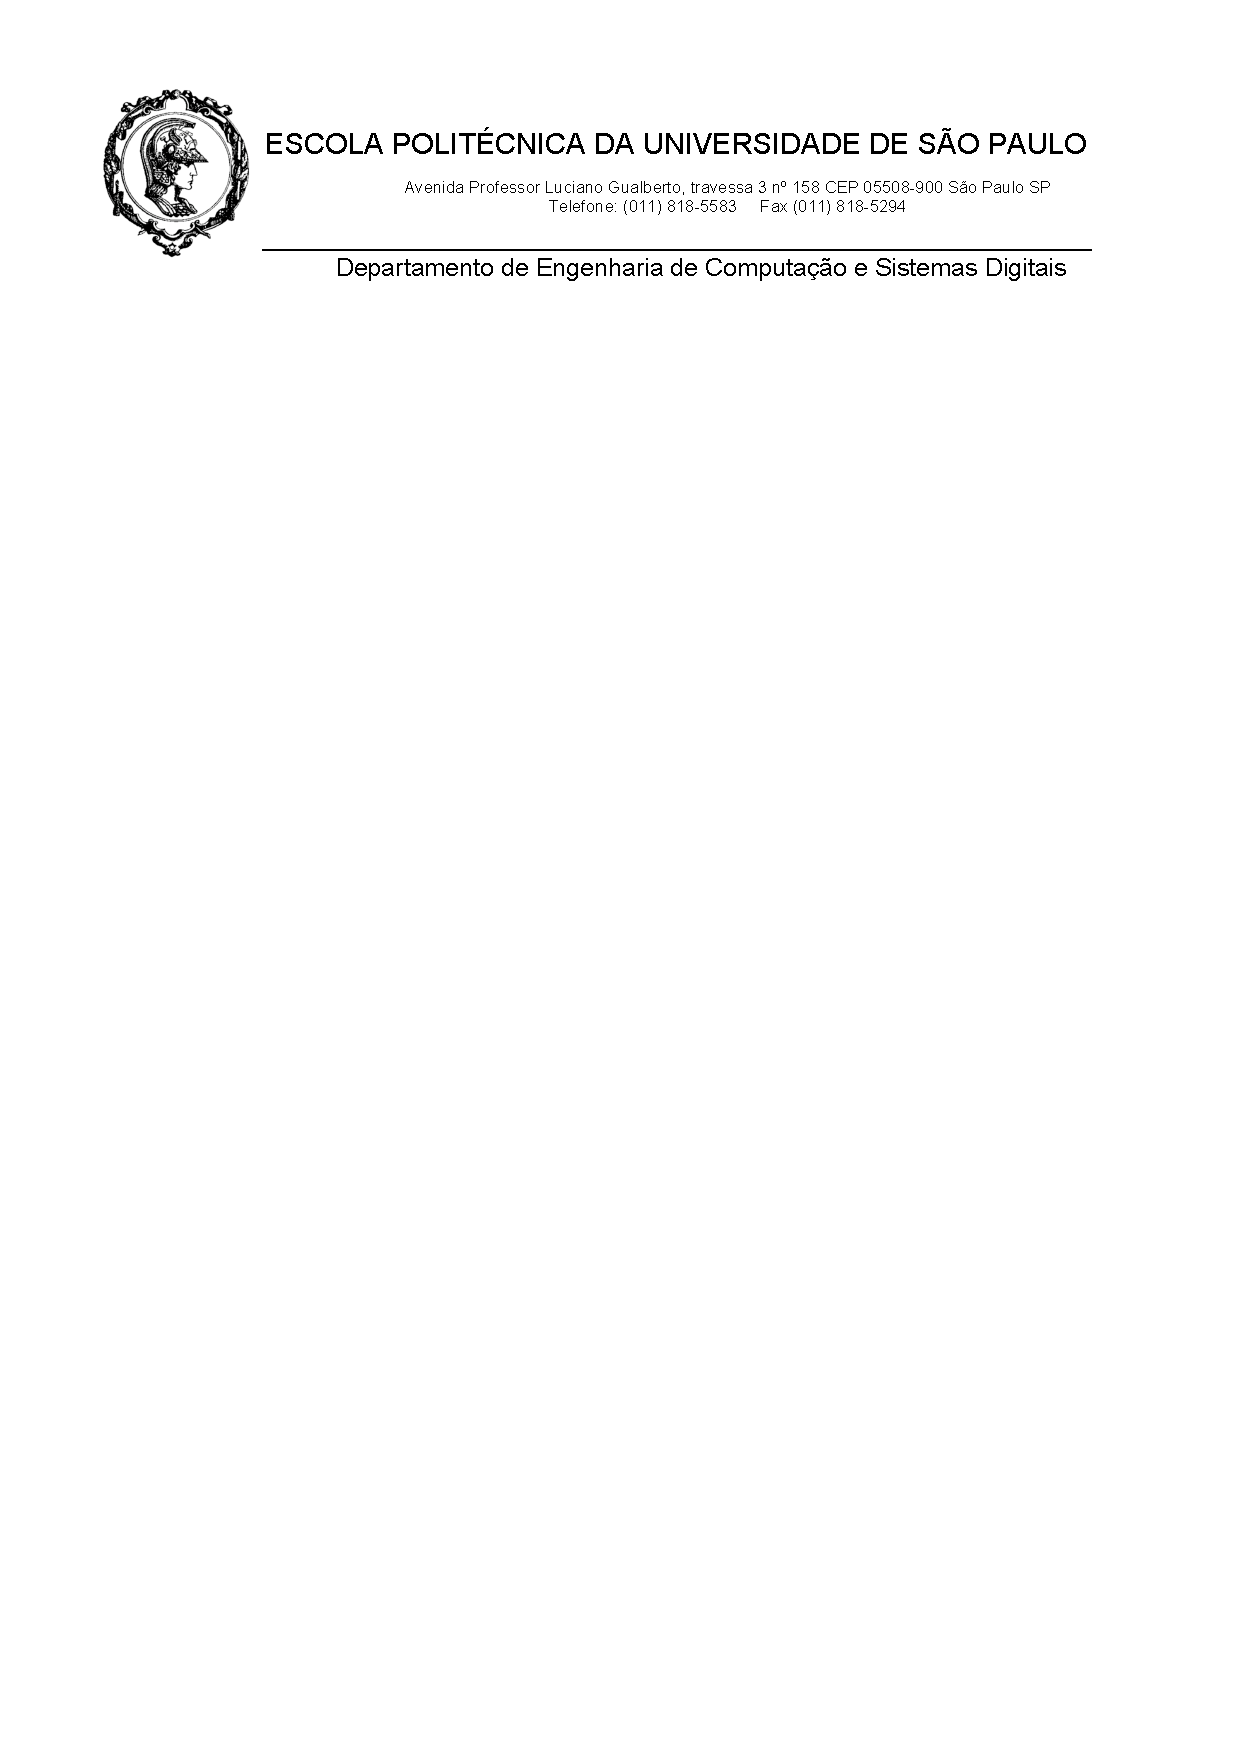
\includegraphics[width=15.5cm]{imagens/logo.pdf}
\end{figure}

\maketitle

\setlength{\parskip}{0cm}
\tableofcontents
\setlength{\parskip}{\baselineskip}
\chapter{Introdu��o}

Desde a publica��o por Alan Turing, em 1936, da sua M�quina de Turing capaz de computar qualquer fun��o efetivamente comput�vel buscou-se construir formas ou t�cnicas para resolver os problemas dif�ceis atrav�s do computador. O campo da Intelig�ncia Artificial apresenta algumas t�cnicas e algoritmos para solu��o computacional desses problemas de grande complexidade, muitas vezes sem a garantia da solu��o �tima, mas resultados, na maioria das vezes, satisfat�rios.

O SAURON � um rob� m�vel projetado para guiar pessoas em museus. Ele utiliza t�cnicas de IA para conseguir navegar e se localizar em um ambiente conhecido, problema de grande complexidade. Esta monografia � parte do trabalho de conclus�o do curso de Engenharia de Computa��o da Escola Polit�cnica da Universidade de S�o Paulo (POLI). Como demonstra��o pr�tica, o SAURON guiar� os visitantes pelo pr�dio da �rea de El�trica da POLI.

Para possibilitar a tarefa de localiza��o, o SAURON deve coletar informa��es acerca de si e do ambiente ao seu redor utilizando seus sensores: od�metro, sonares e c�mera de v�deo de baixo custo. Essas informa��es coletadas devem ser suficientes para determinar sua pr�pria localiza��o nesse ambiente.

A t�cnica principal empregada na determina��o de sua localiza��o � um filtro Bayesiano conhecido por filtro de Kalman estendido (EKF). Os filtros bayesianos s�o criados a partir da teoria de Bayes, a partir da qual � poss�vel estimar a probabilidade de um determinado evento, dado que um segundo evento tenha ocorrido. Os filtros bayesianos aplicados ao problema de localiza��o s�o capazes de apurar uma nova estimativa de posi��o a partir da estimativa anterior.

Outro problema dif�cil � a navega��o por um ambiente. � necess�rio um sistema que atinja os objetivos especificados pelo visistante de forma segura, mantendo-se afastado de objetos e pessoas. O SAURON ainda � capaz de navegar entre m�ltiplos mapas, o que possibilita a utiliza�ao do rob� em um ambiente com mais de um andar. Esses dois planejadores, inter e intra mapas, utilizam, cada um, t�cnicas diferentes para escolha da melhor rota: enquanto o planejador de rota de um �nico mapa deve lidar com diversos pontos naveg�veis em um mapa e deve garantir a escolha do melhor caminho, o planejador de rota entre mapas pode ser simplista, pois sabe-se que, durante sua utiliza��o, ele ficar� restrito a dois ou tr�s mapas distintos.

A navega��o inclui tamb�m uma camada de execu��o de rota, que al�m de controlar o caminho percorrido, deve evitar colis�es do rob� com obst�culos. O ambiente para o qual o SAURON foi projetado � um museu, assim, ao evitar obst�culos o SAURON est� preservando as obras de arte do museu, mas, acima de tudo, preservando a integridade f�sica dos visitantes. 

Ao longo deste trabalho, o sistema completo do SAURON ser� descrito e os problemas incipientes da localiza��o e da navega��o ser�o tratados em maiores detalhes.



\section{Objetivo}

O objetivo deste trabalho � a constru��o de um rob� que seja capaz de guiar visitantes em ambientes fechados. A aplica��o t�pica dessa classe de agentes � o acompanhamento de visitantes em exposi��es, como fazem \cite{Burgard98experienceswith}, \cite{Thrun99minerva} e \cite{Siegwart02largescale}. Para alcan�ar seus objetivos, esse rob� deve ser capaz de efetuar:
\begin{itemize}
  \item localiza��o em seu mapa interno;
  \item planejamento de rota para seu destino final partindo de sua localiza��o;
  \item navega��o pelo ambiente cumprindo a rota planejada;
  \item desvio ou detec��o de obst�culos din�micos.
\end{itemize}

Para que realize essas a��es, um agente m�vel deve extrair informa��es sensoriais de seu estado atual, e relacion�-las com seu conhecimento do ambiente. Um dos motivadores deste trabalho � a constru��o de um rob� de baixo custo. Nesse sentido, s�o utilizados, como sensores, um anel de oito sonares e uma c�mera de v�deo dom�stica. Em rela��o ao encontrado na literatura, em que or�amentos para tarefas semelhantes ultrapassam as centenas de milhares de d�lares \cite{Siegwart02largescale}, o projeto apresentado neste texto � ordens de grandeza mais barato.

As t�cnicas de localiza��o utilizadas neste trabalho s�o adaptadas de \cite{barra}. O planejamento da rota � feito utilizando-se o algoritmo de busca A*, e a navega��o busca criar rotas retas, adequadas ao bom funcionamento do sistema de localiza��o.

\section{Organiza��o do trabalho}
O restante deste trabalho est� dividido da seguinte forma: 

O cap�tulo \ref{sec:revisaoLiteratura}, Revis�o da literatura, apresenta o resultado da pesquisa bibliogr�fica realizada sobre rob�s aut�nomos e rob�s-guias. O cap�tulo \ref{subsec:arquitetura} apresenta como foi definida a arquitetura de software do SAURON, descrevendo o sistema de localiza��o e navega��o desenvolvidos. No cap�tulo \ref{subsec:modelodinamica} � discutido o modelo de din�mica adotado. O cap�tulo \ref{subsec:modelosonares} detalha o m�dulo de sonar utilizado no SAURON, descrevendo dois m�todos desenvolvidos para utiliza��o em localiza��o. Ap�s isto, no cap�tulo \ref{subsec:modeloVisao} � detalhado o modelo de vis�o desenvolvido. No cap�tulo \ref{sec:resultados} � explicado a metodologia de testes utilizadas e s�o exibidos os resultados dos testes realizados, tanto com o simulador como com o rob� f�sico. Por fim, no cap�tulo \ref{sec:discussao} � apresentada uma discuss�o sobre os m�todos desenvolvidos, seus custos e resultados.

Finalmente, no cap�tulo \ref{chp:Conclusoes} � apresentada a conclus�o do trabalho, seguida no cap�tulo 4 pela bibliografia utilizada durante o trabalho. Ap�s isto h� um ap�ndice onde � tratado com maiores detalhes o filtro de kalman discreto e o EKF, variante utilizada no presente trabalho.
\section{Progressos}

Como foi especificado no documento de especifica��o, n�s seguiremos a arquitetura indicada na figura~\ref{arquitetura:global} abaixo.

\begin{figure}[h]%
\begin{center}
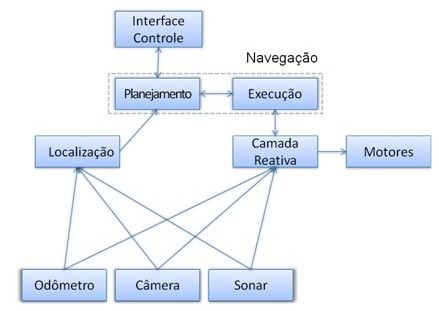
\includegraphics[width=.5\columnwidth]{imagens/arquitetura.jpg}
\caption{Arquitetura do Sistema completo.}%
\label{arquitetura:global}%
\end{center}
\end{figure}

Od�metros e sonares s�o sensores presentes na plataforma-rob� Pionner P2DX. A Vis�o ser� provida por uma c�mera comercial de baixo custo. Nossos testes est�o sendo realizados com a HS988 da Raysun Shine e com a Microsoft LifeCam VX1000.

Nossos progressos concentraram-se no M�dulo de Localiza��o, cuja arquitetura se baseia no uso do estimador bayesiano conhecido por Filtro Estendido de Kalman. A arquitetura detalhada do M�dulo de Localiza��o encontra-se na figura~\ref{arquitetura:localizacao} abaixo.

\begin{figure}[h]%
\begin{center}
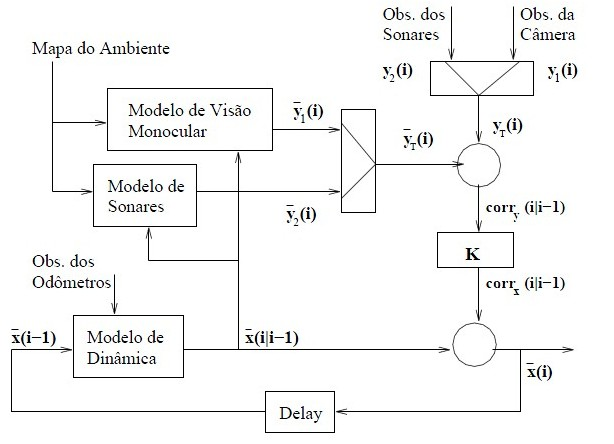
\includegraphics[width=.5\columnwidth]{imagens/arquitetura_localizacao.jpg}
\caption{Arquitetura Detalhada do M�dulo de Localiza��o.\cite{barra}}%
\label{arquitetura:localizacao}%
\end{center}
\end{figure}

Os trabalhos do �ltimo m�s resultaram em um avan�o consider�vel no m�dulo de localiza��o.

\subsection{Arquitetura do Sistema}
Todos os m�dulos do sistema foram integrados, e os testes do sistema completo come�aram. Uma arquitetura de software fortemente ass�ncrona e desacoplada foi desenvolvida, com resultados satisfat�rios. A arquitetura do sistema � descrita na se��o \ref{sec:arquitetura}.

\subsection{Filtro Estendido de Kalman (EKF)}
O c�digo do filtro estendido de Kalman, EKF, foi implementado e testado no simulador.

\subsection{Modelo de Din�mica}
O modelo de din�mica foi finalizado e testado no simulador. Ele � descrito na se��o \ref{sec:dinamica}.

\subsection{Modelo de Sonares}
O modelo de sonares foi finalizado e testado no simulador. Muito esfor�o foi gasto para garantir que a modelagem matem�tica dos sonares estava correta. As equa��es finais podem ser vistas na se��o \ref{sec:sonar}.

\subsection{Modelo de Vis�o}
Se��o \ref{sec:visao}.
\begin{comment}
\documentclass[a4paper,11pt]{article}
\usepackage{graphicx}
\usepackage[brazilian]{babel}
\usepackage[latin1]{inputenc}
\usepackage[T1]{fontenc}
\usepackage{fullpage}
\begin{document}
\end{comment}

\section{Testes com a biblioteca SonARNL}

A empresa MobileRobots, fabricante do rob� Pioneer P2DX utilizado no projeto, disponibiliza a seus clientes uma biblioteca chamada SonARNL, que prov� fun��es de localiza��o e navega��o rob�ticas. O c�digo-fonte da biblioteca � fechado, e alguns exemplos em C++ distribu�dos no pacote ensinam como utiliz�-la.

A primeira abordagem em busca da realiza��o do m�dulo de Localiza��o foi a tentativa de incorporar a biblioteca SonARNL dentro de nosso sistema, o que nos economizaria muito tempo de desenvolvimento.

\subsection{Ambiente de testes}
Testamos o rob� em duas ocasi�es. No primeiro dia, montamos um circuito assim�trico e pequeno, que ia da sala C2-50 ao corredor que termina nas escadas. Para aumentar a assimetria, modificamos o ambiente original. A Figura~\ref{mapa:testesonarnl1} representa o ambiente de testes.
\begin{figure}[h]%
\begin{center}
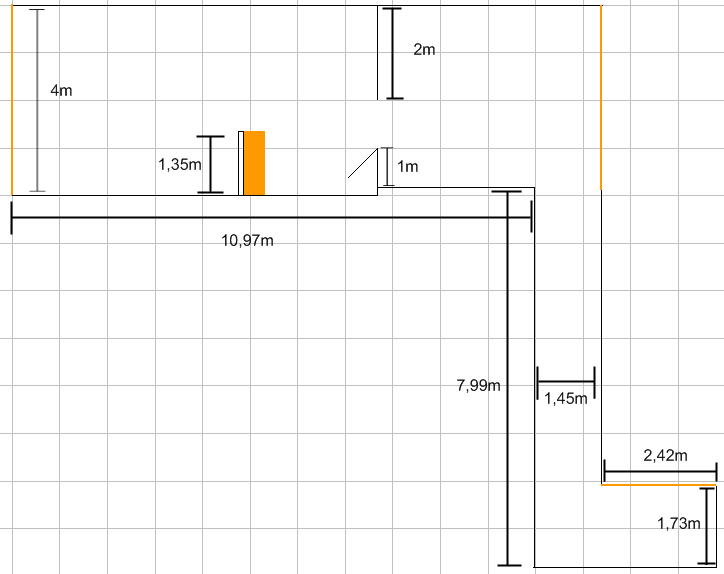
\includegraphics[width=.5\columnwidth]{imagens/mapa.png}
\caption{Mapa do primeiro dia de testes}%
\label{mapa:testesonarnl1}%
\end{center}
\end{figure}

No segundo dia, testamos a capacidade do rob� de se deslocar por todo o pavimento superior do bloco C, local escolhido por representar desafios comuns a todo o ambiente, em especial, alta simetria entre as duas paredes do corredor. Para mapearmos o ambiente, obtivemos uma planta, no formato AutoCAD, de todo o pr�dio, que havia sido constru�da por ex-alunos da Prof. Anna. O resultado est� ilustrado na Figura~\ref{mapa:testesonarnl2}. Convertemos a parte dessa planta que nos interessava para o formato entendido pela biblioteca SonARNL, e verificamos manualmente a corre��o das medidas. Localizamos algumas imprecis�es (por vezes grosseiras), que foram corrigidas. � medida que os testes progrediram, o mapa foi refinado cada vez mais.

\begin{figure}%
\begin{center}
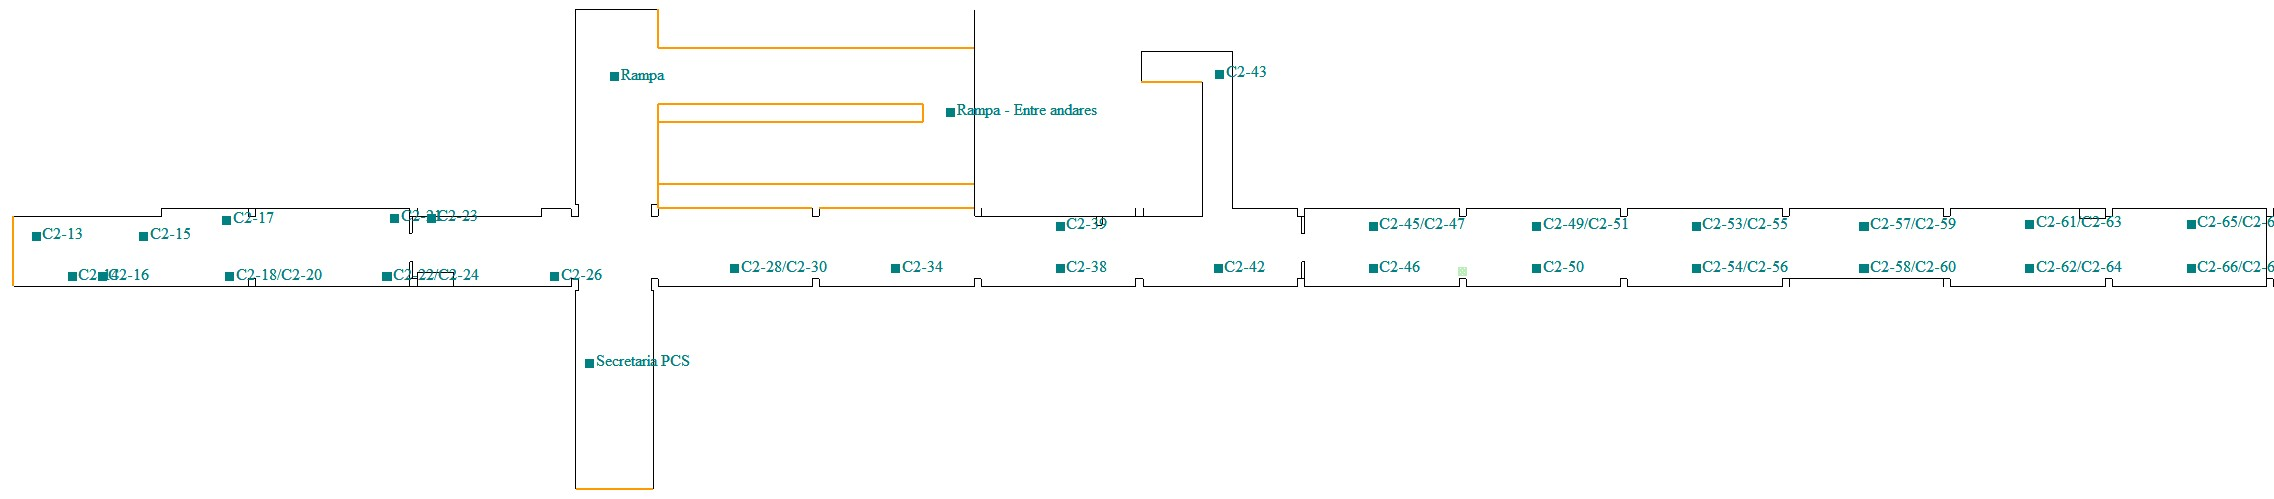
\includegraphics[width=\columnwidth]{imagens/mapa2.jpeg}
\caption{Mapa do segundo dia de testes, com os pontos de interesse. As linhas laranjas representam ``zonas proibidas'', linhas invis�veis aos sensores do rob� mas que devem ser evitadas.}%
\label{mapa:testesonarnl2}%
\end{center}
\end{figure}

\subsection{Resultado dos testes}
No primeiro dia de testes, o rob� foi capaz de se deslocar com sucesso no circuito, atingindo os objetivos selecionados. Para aferir a precis�o do rob�, marcamos 20 pontos no ambiente. O rob� foi instru�do a se dirigir a cada um deles e, quando a biblioteca informava ter atingido seu destino, med�amos o erro entre a posi��o real e a cren�a do rob�.

Foram realizadas tr�s baterias de testes. Nas duas primeiras, o rob� encontrou um ambiente perfeitamente est�tico e o erro m�dio foi de 30,18 cent�metros. No �ltimo teste, tentamos atrapalh�-lo, ficando na frente dos sonares. A diferen�a nos resultados foi percept�vel: o erro m�dio subiu para 90,62 cent�metros, e por quatro vezes o rob� colidiu com pessoas ou paredes.

No segundo dia de testes, o pavimento superior inteiro foi utilizado como mapa. O ambiente, bastante sim�trico, n�o foi modificado, o que aumentou a dificuldade de localiza��o. Nessas novas condi��es, a biblioteca SonARNL n�o foi capaz de atingir os destinos. De fato, ele n�o foi capaz de se locomover em linha reta da sala C2-50 � C2-13. Na tentavia de compreender os motivos do erro, tentamos alterar alguns par�metros (por exemplo, n�mero de amostras do algoritmo Monte Carlo), sem sucesso. Detectamos um padr�o interessante: na maior parte das vezes em que se perdeu, o rob� acreditava estar no lado errado do corredor. Por exemplo, ele achava estar pr�ximo � parede da sala C2-30, quando na verdade estava encostado � rampa oposta.

Tampouco foram raros os acidentes. Os sonares garantem prote��o contra colis�es frontais, mas muitas vezes o rob�, acreditando estar no lado oposto do corredor, efetuou um giro de 360� quando estava encostado � parede, raspando a al�a traseira e o notebook embarcado.

Notamos que � medida que o mapa era refinado, havia alguma melhora no desempenho do rob�, mas n�o conseguimos um comportamento consistente em hora alguma: se �s vezes ele chegava a ultrapassar o cruzamento dos corredores, no teste seguinte ele poderia muito bem se perder antes da primeira porta de vidro.

\subsection{Avalia��o dos resultados}

Os resultados dos testes foram ruins, j� que a biblioteca de localiza��o do rob� se mostrou incapaz de atingir seu objetivo b�sico. Pior ainda, n�o conseguimos discernir exatamente \emph{o qu�} causava essa imprecis�o. Na tentativa de isolar as causas do erro, realizamos um terceiro dia de testes. Tentamos diminuir a assimetria do ambiente, melhorar a precis�o do mapa e modificar os mais diversos par�metros do algoritmo, mas n�o notamos melhoras no desempenho do rob�.\footnote{Uma grande dificuldade em realizar esses testes � a grande varia��o nos resultados. N�o h� um determinismo claro nas a��es do rob�. Por exemplo, se em um determinado teste o rob� se perdeu perto da sala C2-46, no pr�ximo teste, com condi��es id�nticas, a perda de localiza��o poderia ocorrer muito antes ou depois, sem nenhum motivo aparente. Seria necess�rio um n�mero muito grande de medidas para eliminar as varia��es aleat�rias e determinar o efeito das mudan�as de par�metros.}

Chegamos, finalmente, a um est�gio em que n�o poder examinar o c�digo-fonte da biblioteca foi limitante. Para que pud�ssemos analisar com mais detalhes as raz�es do fracasso da localiza��o, precisar�amos entrar mais fundo nas engrenagens no c�digo. Como isso n�o era poss�vel, tomamos a decis�o de abandonar a biblioteca de localiza��o do SonARNL.


%\end{document}
\begin{comment}
\documentclass[a4paper,11pt]{article}
\usepackage{graphicx}
\usepackage[brazilian]{babel}
\usepackage[latin1]{inputenc}
\usepackage[T1]{fontenc}
\usepackage{fullpage}
\begin{document}
\end{comment}

\section{Modelo de Din�mica}

\subsection{Convolu��o}
The quick brown fox jumps over the lazy dog.

\subsection{Detec��o de Proje��es Verticais}
The quick brown fox jumps over the lazy dog.

\subsection{Perfil de Cor}
The quick brown fox jumps over the lazy dog.

\subsection{Rastreamento e Associa��o}
The quick brown fox jumps over the lazy dog.

\subsection{Pr�ximos Passos}
The quick brown fox jumps over the lazy dog.

% \end{document}
\section{Modelo de Vis�o}
\label{sec:visao}

A vis�o monocular, cujo sensor � uma �nica c�mera de v�deo, permite obter uma boa estimativa da localiza��o do rob� devido a grande quantidade de est�mulos visuais que existem. 

Dentre os v�rios tipos de est�mulos, neste modelo, baseado em \cite{barra}, o principal est�mulo s�o as retas verticais presentes nos ambientes, tais como batentes de portas, colunas, janelas, etc. A denomina��o \textsl{reta vertical} ser� dada �s retas presentes no mundo real enquanto \textsl{proje��es} s�o as observa��es dessas retas nas imagens obtidas pela c�mera.

\subsection{Convolu��o}

A convolu��o � aplicada sobre as imagens para que seja poss�vel ressaltar os cantos de objetos contidos na imagem, de maneira an�loga ao Filtro de Sobel, uma vez que a caracter�stica visual de interesse s�o retas verticais. 

A id�ia b�sica da convolu��o de imagens, que � discreta e bidimensional, � a de uma janela que � deslizada sobre a imagem. O valor do pixel resultante � igual � soma ponderada dos pixels da imagem original que se encontram dentro da janela. Os pesos s�o os valores do filtro que foram estabelecidos para cada um dos pixels da janela. Tal janela � denomindada \textit{kernel} da convolu��o. 

O \textit{kernel} foi determinado empiricamente, considerando-se dois par�metros: precis�o na demarca��o das retas verticais e desempenho, uma vez que aplicar a convolu��o sobre uma imagem � um processo computacionalmente pesado.

\begin{figure}[ht]
	\centering
		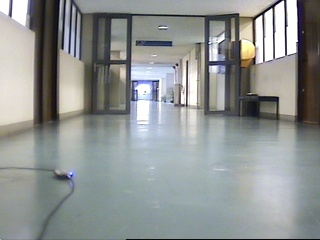
\includegraphics[width=.6\columnwidth]{imagens/corredor.jpg}
	\caption{Foto tirada no corredor das salas C2}%
	\label{visao:original}
\end{figure}

\begin{figure}[ht]
	\centering
		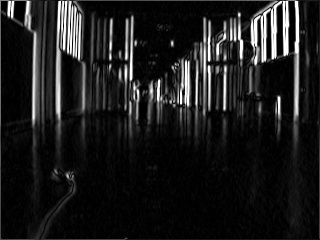
\includegraphics[width=.6\columnwidth]{imagens/sobel.jpg}
	\caption{Imagem obtida ap�s a aplica��o da convolu��o sobre a Figura~\ref{visao:original}}
	\label{visao:convolucao}
\end{figure}


\subsection{Detec��o de Proje��es Verticais}

A detec��o de proje��es � feita sobre a imagem em tons de cinza resultante da convolu��o do filtro para linhas verticais e tem como objetivo converter as linhas desenhadas para uma estrutura de dados que permita novas formas de manipula��o dos dados.

%Antes de iniciar a detec��o, aplica-se um procedimento que filtra pixels que n�o s�o m�ximos locais, isto �, dada uma pequena por��o da imagem, a intensidade n�o � a maior dessa regi�o. J� que a tend�ncia do filtro de convolu��o usado � marcar os pixels mais perto do centro de uma linha vertical com valores maiores que os pixels perif�ricos da mesma linha, o procedimento aplicado faz com que uma poss�vel proje��o, antes representada na imagem como uma linha relativamente grossa (v�rios pixels), passe a ter largura de um �nico pixel.

Ela � iniciada em um estado no qual a imagem � varrida, da esquerda para a direita, de cima para baixo, buscando um pixel que tenha intensidade maior do que um \textsl{limiar de in�cio}. Quando um pixel atende a esse requisito, passa-se a um estado secund�rio.

Neste novo estado, supoe-se que o pixel acima do limiar � um ponto de um nova proje��o. A partir dele, a imagem passa a ser varrida verticalmente, da seguinte forma: compara-se o valor dos tr�s pixels vizinhos que est�o abaixo do pixel rec�m-inserido na nova poss�vel proje��o. O pixel que ser� adicionado na proje��o ser� aquele com o maior valor. Este processo engloba algumas heur�sticas que levam � obten��o das proje��es mais significativas para as etapas posteriores, al�m de filtragem por tamanho da proje��o, eliminando, assim, proje��es muito pequenas, e a inclina��o, descartando aquelas que n�o est�o t�o verticais quanto desejado.


% mas exitem algumas ressalvas: 
%\begin{itemize}
%\item se o pixel de maior valor for um dos inferiores laterais, entra em a��o um fator de in�rcia vertical cujo papel � for�ar a proje��o a ser o mais vertical poss�vel. Enquanto este fator estiver ativo, � dada prefer�ncia para o pixel diretamente abaixo, mesmo que seu valor n�o seja o maior. Esse fator ser� desativado quando alguns pixels n�o m�ximos forem selecionados, evitando a forma��o de um proje��o distorcida.
%\item se o maior valor for inferior a um limiar de t�rmino, o pixel � adicionado temporariamente � proje��o e passa-se a contar quantos pixels abaixo do limiar foram inseridos em seq��ncia. Caso essa contagem ultrapasse um valor m�ximo, todos os que foram adicionados temporariamente s�o removidos, a proje��o obtida at� ent�o � considerada finalizada e o algoritmo de detec��o volta ao estado inicial. Se ap�s alguns pixels abaixo do limiar de t�rmino serem inseridos, mas com contagem menor do que a m�xima permitida, for encontrado um pixel cuja intensidade � superior ao limiar de t�rmino, a adi��o deles � confirmada e a contagem � zerada.
%\end{itemize}

%Cada proje��o detectada passa por algumas verifica��es que incluem o tamanho da proje��o, eliminando, assim, proje��es muito pequenas, e a inclina��o, descartando aquelas que n�o est�o t�o verticais quanto desejado.

\begin{figure}[h]
	\centering
		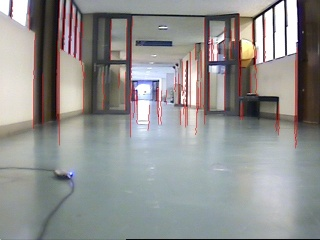
\includegraphics[width=.6\columnwidth]{imagens/projections.jpg}
	\caption{Proje��es detectadas na Figura ~\ref{visao:original}}
	\label{visao:projecoes}
\end{figure}


\subsection{Perfil de Cor}
O perfil de cor segue a hip�tese que a distribui��o de cores ao redor das retas verticais cont�m informa��o suficiente para ajudar a identificar proje��es de uma mesma reta vertical em diferentes quadros do v�deo.

Ele considera uma regi�o da imagem centrada na seq��ncia de pixels que pertencem a uma proje��o identificada, estendendo-se por uma faixa de \textit{n} pixels para a direita e para a esquerda de cada pixel da proje��o.

As informa��es que se mostraram relevantes sobre o perfil de cor s�o os valores m�dios, para cada componente de cor, dos lados esquerdo e direito em rela��o ao centro da regi�o.

A compara��o de dois perfis de cor, logo, de duas proje��es, resulta num fator de correla��o normalizado que indica qu�o semelhantes s�o os perfis. O c�lculo desse fator segue as seguintes equa��es:

\begin{eqnarray*}
R & = & \left( \delta - \vert R_{1_{esq}} - R_{2_{esq}} \vert \right) + \left( \delta - \vert R_{1_{dir}} - R_{2_{dir}} \vert \right) \\
G & = & \left( \delta - \vert G_{1_{esq}} - G_{2_{esq}} \vert \right) + \left( \delta - \vert G_{1_{dir}} - G_{2_{dir}} \vert \right) \\
B & = & \left( \delta - \vert B_{1_{esq}} - B_{2_{esq}} \vert \right) + \left( \delta - \vert B_{1_{dir}} - B_{2_{dir}} \vert \right)
\end{eqnarray*}
\begin{displaymath}
C = \frac{\left( R + G + B \right)}{6\delta} 
\end{displaymath}


onde $\delta$ � a maior diferen�a esperada entre os componentes, $R$, $G$ e $B$ s�o representam as diferen�as nas intensidades dos componentes de cor entre o lado direito e esquerdo, em rela��o � reta considerada, e $C$ � o fator de correla��o. Esse modelo n�o � o usado originalmente por Barra\cite{barra}, pois o usado por ele apresentou resultados ruins nos testes realizados. O motivo de tais resultados parece decorrer do fato de seu modelo considerar as m�dias das diferen�as entre os valores de cada lado da reta. Os testes revelaram que isso leva v�rios perfis distintos a possu�rem valores muito pr�ximos, e, consequentemente, a v�rias falsas correla��es.

Esta nova modelagem foi escrita visando considerar diferen�as de um mesmo lado da regi�o, para cada componente de cor, aumentando o valor do fator de correla��o quando as cores de cada lados dos perfis comparados s�o pr�ximos. 

\subsection{Rastreamento e Associa��o}
A associa��o de proje��es � marcos foi dividida em duas etapas: rastrear proje��es em seq��ncias cont�nuas de quadros e relacionar proje��es rastreadas � marcos descritos no mapa. 

%Essa abordagem n�o � a mesma seguida por Barra\cite{barra}, que busca a melhor associa��o aos marcos usando todas as proje��es observadas em um dado instante. Maiores detalhes sobre os motivos da divis�o ser�o citados abaixo.

O rastreamento de proje��es � respons�vel por identificar proje��es em diferentes quadros que s�o, na verdade, a mesma proje��o vista em um momento e/ou posi��o diferente. A import�ncia dessa etapa � que ela realiza uma filtragem pelas proje��es que t�m maior probabilidade de serem marcos. Isso decorre das caracter�sticas desejadas em marcos: altamente vis�veis e facilmente identific�veis. Se uma mesma proje��o pode ser vista por muito tempo, ela pode ser um marco. 
%Dessa forma, o rastreamento tamb�m age de maneira an�loga ao buffer adotado por Barra\cite{barra}.

O rastreamento � feito a partir da compara��o dos perfis de cor entre as proje��es que foram observadas no �ltimo quadro obtido da c�mera com aquelas que foram vistas em quadros anteriores, fazendo uso do valor de correla��o explicado na se��o anterior. Com isso, consegue-se determinar qual proje��o nova representa uma antiga no instante de tempo atual, sendo poss�vel manter um hist�rico das diferentes proje��es, que s�o na verdade a mesma observada em tempos diferentes.

%A implementa��o do rastreamento � iniciada com a compara��o de todas as proje��es que est�o sendo rastreadas com todas as que acabaram de ser detectadas no �ltimo frame obtido da c�mera. Essa compara��o, baseada no perfil de cor, resulta num valor de correla��o. Somente os valores acima de um dado limiar, determinado empiricamente, s�o aceitos. Em seguida, os valores s�o agrupados de acordo com a proje��o rastreada que foi usada para ger�-lo, e ordenados, em ordem decrescente. Para cada grupo, calcula-se um fator de similaridade. O grupo que tiver o maior valor de similaridade, ter� o direito de utilizar a proje��o rec�m-observada, associada ao maior valor de correla��o, para relacionar � sua proje��o rastreada. Ap�s isso, o grupo com maior similaridade � removido, assim como todos os valores de correla��o, dos demais grupos, associados � proje��o rec�m-observada que foi usada. O c�luclo de similaridade e a busca pelos grupos � repetida at� que todas as proje��es rastredas sejam relacionadas ou que ou o maior valor de similaridade encontrado esteja abaixo de um limiar.

%O efeito de buffer se deve ao fato do rastreador poder ser configurado para considerar que uma dada proje��o s� est� sendo devidamente rastreada se ela for vista pelos n vezes nos �ltimos i quadros, sendo n e i facilmente ajust�veis.

A associa��o de marcos � feita entre proje��es rastreadas e marcos descritos num arquivo. Um marco foi modelado como um perfil de cor que se encontra em uma determinada coordenada $\left(x, y\right)$ do mundo real. O algoritmo de associa��o de marcos, segue, em ess�ncia, as mesmas id�ias aplicadas no rastreamento de proje��es, existindo apenas diferen�as quanto as estruturas de dados empregadas na implementa��o do algoritmo. 

\subsection{Implementa��o}
Todos as etapas descritas acima j� foram implementadas e testadas em situa��es reais, mas de menor escala, tendo resultados bastante satisfat�rios, revelando, apenas, a necessidade de pequenos refinamentos. Infelizmente, n�o � poss�vel automatizar os testes do m�dulo de vis�o dada a dificuldade em criar um mecanismo de avalia��o dos resultados, o que seria algo t�o trabalhoso quanto o pr�prio desenvolvimento do m�dulo.

Atualmente, o m�dulo de vis�o se encontra em \textsl{stand-by}, at� que a possa ser feita a integra��o com o filtro de Kalman.

\subsection{Pr�ximos Passos}
A prioridade do componente de vis�o � a implementa��o do estimador que alimentar� o Filtro de Kalman. Como o filtro ainda est� para ser desenvolvido, decidiu-se aguardar at� que sua interface esteja consolidada o suficiente para que se fa�a o estimador, evitando-se desperd�cio de esfor�o, numa eventual mudan�a nos planos.

Dentre melhorias a serem feitas, h� a inclus�o de um algoritmo que auxilia na associa��o de marcos por meio de estimativas da posi��o que um determinado marco deveria ocupar num frame, conhecendo a postura atual do rob� (posi��o e orienta��o). Entretanto, isso s� pode ser realizado em um est�gio mais avan�ado, devido as depend�ncias que esta melhoria tem como outro m�dulos do projeto.

%\begin{comment}
\documentclass[a4paper,11pt]{article}
\usepackage{graphicx}
\usepackage[brazilian]{babel}
\usepackage[latin1]{inputenc}
\usepackage[T1]{fontenc}
\usepackage{fullpage}
\begin{document}

\begin{equation}
h(x) = \frac{R_{wall} - x_{sonar}\cos \theta_{wall} - y_{sonar}\sin \theta_{wall}}{\sin(\theta'_{sonar} + \theta_{wall} - \theta + \frac{\pi}{2})}
\end{equation}

\begin{equation}
h(x) = \frac{R_{wall} - (x + x'_{sonar} \cos \theta - y'_{sonar} \sin \theta)\cos \theta_{wall} - (y + x'_{sonar} \sin \theta + y'_{sonar} \cos \theta)\sin \theta_{wall}}{\sin(\theta'_{sonar} + \theta_{wall} - \theta + \frac{\pi}{2})}
\end{equation}
\end{comment}


\section{Modelo de Observa��o dos Sonares}
O sonar � um sensor de profundidade que emite ondas sonoras e, a partir do tempo entre emiss�o e recep��o, calcula a dist�ncia ao obst�culo mais pr�ximo. Ele opera de maneira similar a um sensor laser, mas com menor precis�o e densidade. Contudo, um sensor laser � muito caro para algumas aplica��es\footnote{A MobileRobots vende o kit de \textit{upgrade} de rob�s existentes para sensores laser por US\$1 295 (pre�o de desconto para universidades).}. Um dos objetivos de nosso projeto � construir um rob� de baixo custo, utilizando sensores simples, de modo que a escolha do sonar se faz adequada.

A abordagem adotada � fortemente baseada em \cite{barra}. Nesse trabalho, o autor utilizou um modelo de observa��o para os sonares que lhe permitiu localizar rob�s m�veis em um ambiente similar ao contemplado neste projeto. Algumas mudan�as, contudo, foram realizadas no modelo matem�tico.

\subsection{Vis�o geral}

O modelo de observa��o dos sonares � um dos m�dulos de localiza��o do sistema. A sa�da de todos os m�dulos de localiza��o � dirigida ao estimador, que, no nosso caso, � um filtro de Kalman. Cada m�dulo deve fornecer ao filtro as observa��es que seriam esperadas caso o rob� realmente estivesse na posi��o estimada.

De modo geral, a opera��o do modelo dos sonares pode ser dividida em tr�s etapas. Primeiramente, as observa��es s�o validadas e � determinado se estamos realmente enxergando uma parede. Caso estejamos, consultamos o mapa do ambiente e obtemos a posi��o global da parede observada, e, por fim, retornamos a observa��o que seria esperada para aquela parede, supondo que a posi��o estimada do rob� est� correta. Cada sonar � tratado como um sensor isolado.

\paragraph{Valida��o das observa��es} As �ltimas $k$ observa��es s�o consultadas, juntamente com a postura estimada em cada uma delas. Determina-se, com aux�lio do mapa, se as observa��es podem corresponder a uma superf�cie plana. Caso isso seja verdade, estima-se a posu��o da parede.

\paragraph{Associa��o das observa��es com o mapa} O mapa � ent�o consultado para encontrar uma parede que corresponda �s observa��es validadas. Essa associa��o, por ser muito importante, � bastante conservadora. Se o algoritmo de correspond�ncia encontrar uma, e somente uma, parede que corresponda �s leituras do sonar, a associa��o � realizada com sucesso.

\paragraph{Obten��o das observa��es esperadas} De posse da parede que o sonar est� enxergando e da postura estimada do rob�, retorna-se a leitura esperada do sonar.\\

A descri��o detalhada de cada etapa est� fora do escopo deste documento de evolu��o. Ateremo-nos aos refinamentos feitos ao modelo original descrito em \cite{barra}.

\subsection{Detalhamento do modelo}

Definimos $k$ como o n�mero de observa��es obtidas pelo sonar, e $k_{min}$ como o n�mero de observa��es m�nimos para que seja poss�vel a valida��o de uma superf�cie plana. Enquanto $k<k_{min}$ a valida��o falhar�, pois n�o h� dados suficientes para a valida��o dos dados. Quando $k=k_{min}$, inicia-se o processo de valida��o.

Para determinar se as �tlimas \textit{k} observa��es correspondem a uma parede, o modelo original calcula a rela��o entre a diferen�a entre observa��es sucessivas e a dist�ncia percorrida pelo rob� entre elas. A Figura~\ref{barra_modelosonar} ilustra um rob� se dirigindo � parede com �ngulo $\alpha$. Note que os raios dos sonares incidem sempre perpendicularmente � parede, uma suposi��o inveross�mel. Na realidade, os raios dos sonares refletir�o na parede com um determinado �ngulo, que depende de cada sonar ($\theta'_{sonar}$).\footnote{Essa � uma aproxima��o. Um modelo mais preciso para o comportamento dos sonares � um cone de �ngulo $\gamma$, cujo eixo central est� a $\theta_{sonar}$ da origem.}

\begin{figure}
	\centering
		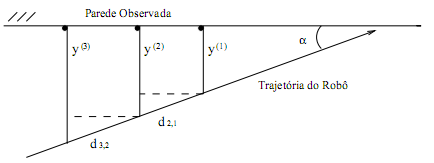
\includegraphics[width=.8\columnwidth]{imagens/sonarbarra.png}
	\caption{Modelo de incid�ncia dos sonares de \cite{barra}}
	\label{barra_modelosonar}
\end{figure}
\begin{figure}
	\centering
		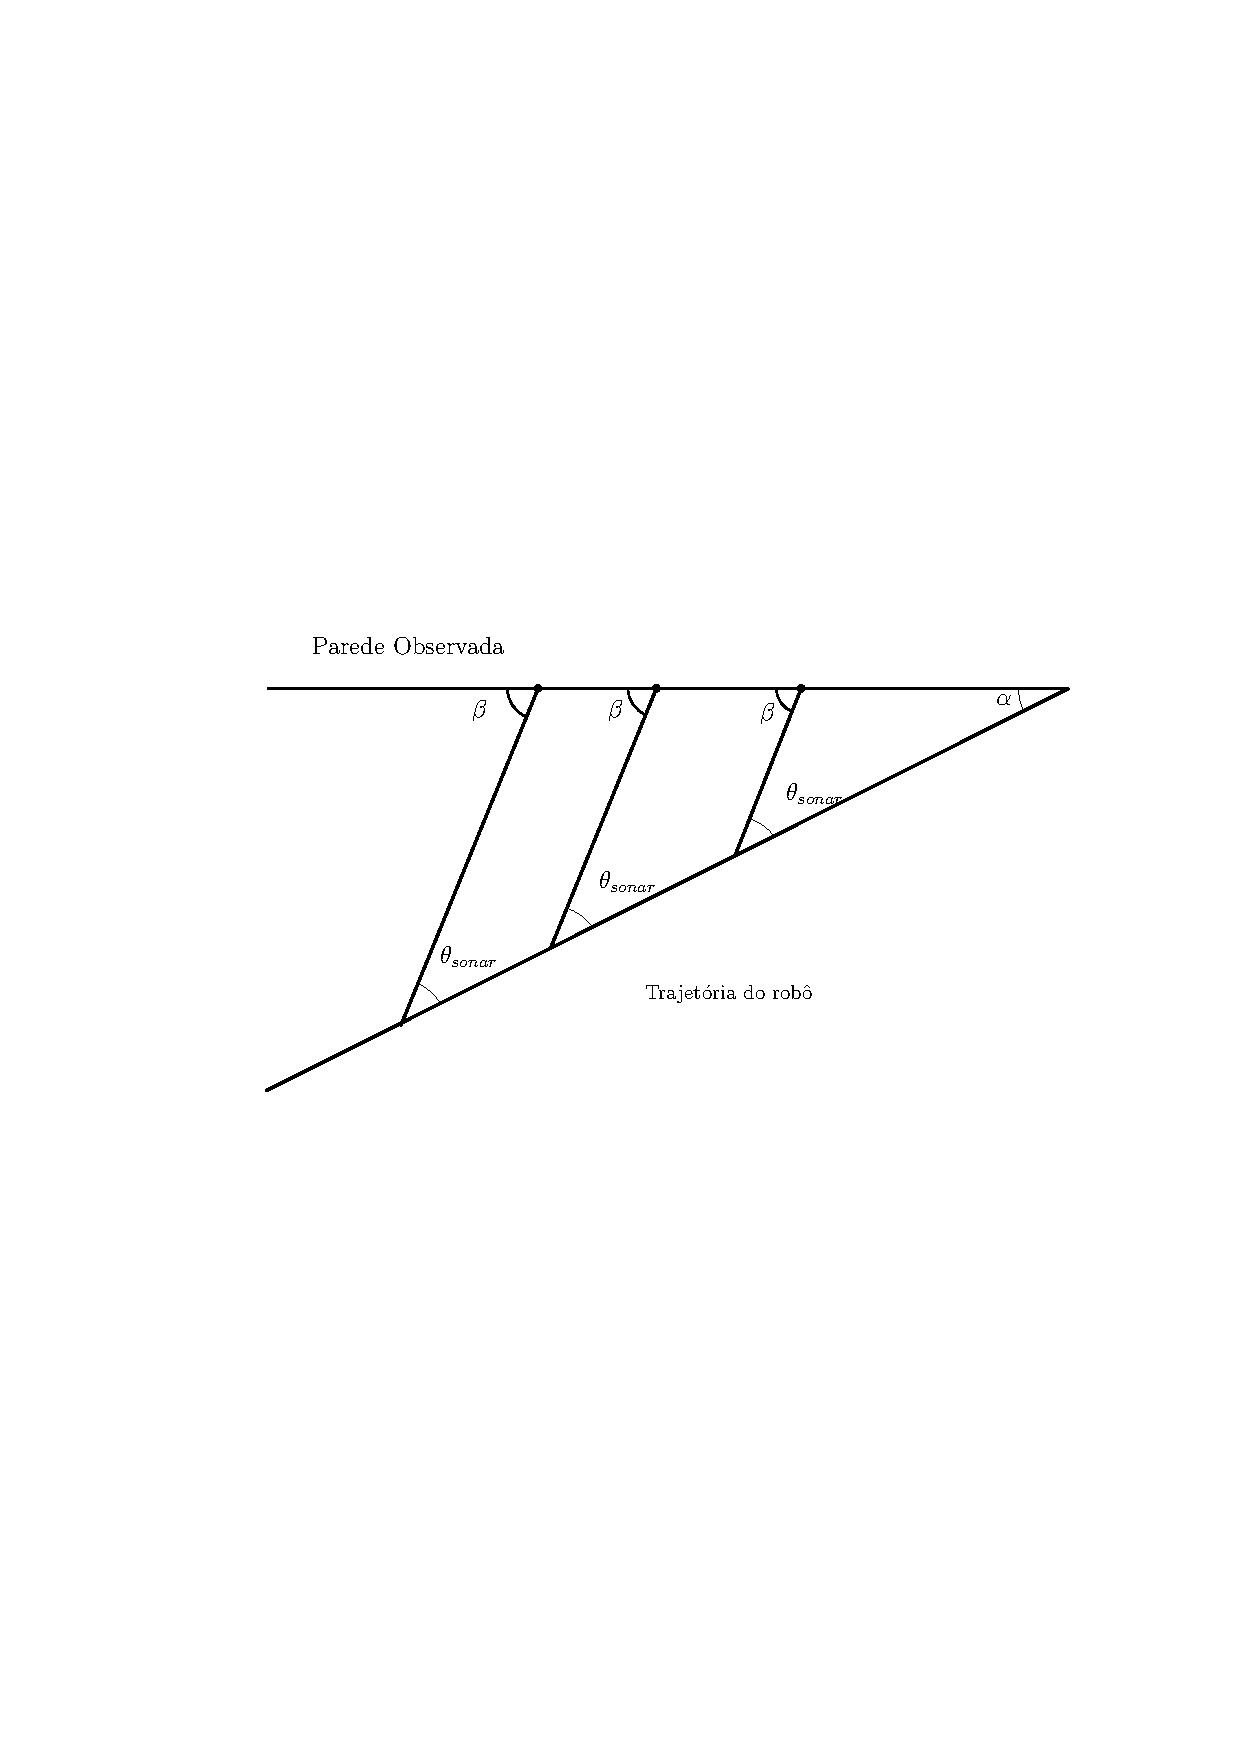
\includegraphics[width=.5\columnwidth]{imagens/nossosonar.pdf}
	\caption{Modelo refinado de incid�ncia dos sonares. $\beta=\theta_{sonar}+\alpha$}
	\label{fig:nossomodelo}
\end{figure}

As equa��es para encontrar $\alpha$ e $r_{wall}$, a dist�ncia da parede at� a origem e $r_{esperada}$, a observa��o esperada do sonar, foram modificadas para refletir o novo modelo:

\begin{equation}
\sin \alpha=\frac{\Delta_{sonar}\sin \theta'_{sonar}}{\sqrt{\Delta_{sonar}^2 + \Delta_{robo}^2 - 2\Delta_{sonar} \Delta_{robo} \cos \theta'_{sonar}}}
\label{eq:novoalpha}
\end{equation}

\begin{equation}
r_{wall}=r\sin\beta+x_{sonar}\cos\theta_{wall}+y_{sonar}\cos\theta_{wall}
\label{eq:novorwall}
\end{equation}

\begin{equation}
r_{esperado}=\frac{r_{wall}-x_{sonar}\cos\theta_{wall}+y_{sonar}\cos\theta_{wall}}{\sin\beta}
\label{eq:novoresperado}
\end{equation}

Nas equa��es acima, $\beta$ � o �ngulo de incid�ncia do raio do sonar, $\Delta_{sonar}$ � a diferen�a entre as leituras do sonar na primeira e �ltima observa��es consideradas v�lidas, $\Delta_{robo}$ � a dist�ncia percorrida pelo rob� entre essas observa��es, $\theta'_{sonar}$ � o �ngulo do sonar em rela��o ao centro do rob� e $\theta_{wall}$ � o �ngulo entre a reta que liga a parede � origem e o eixo $x$. A Figura~\ref{fig:retas} ilustra algumas dessas conven��es.

\begin{figure}
	\centering
	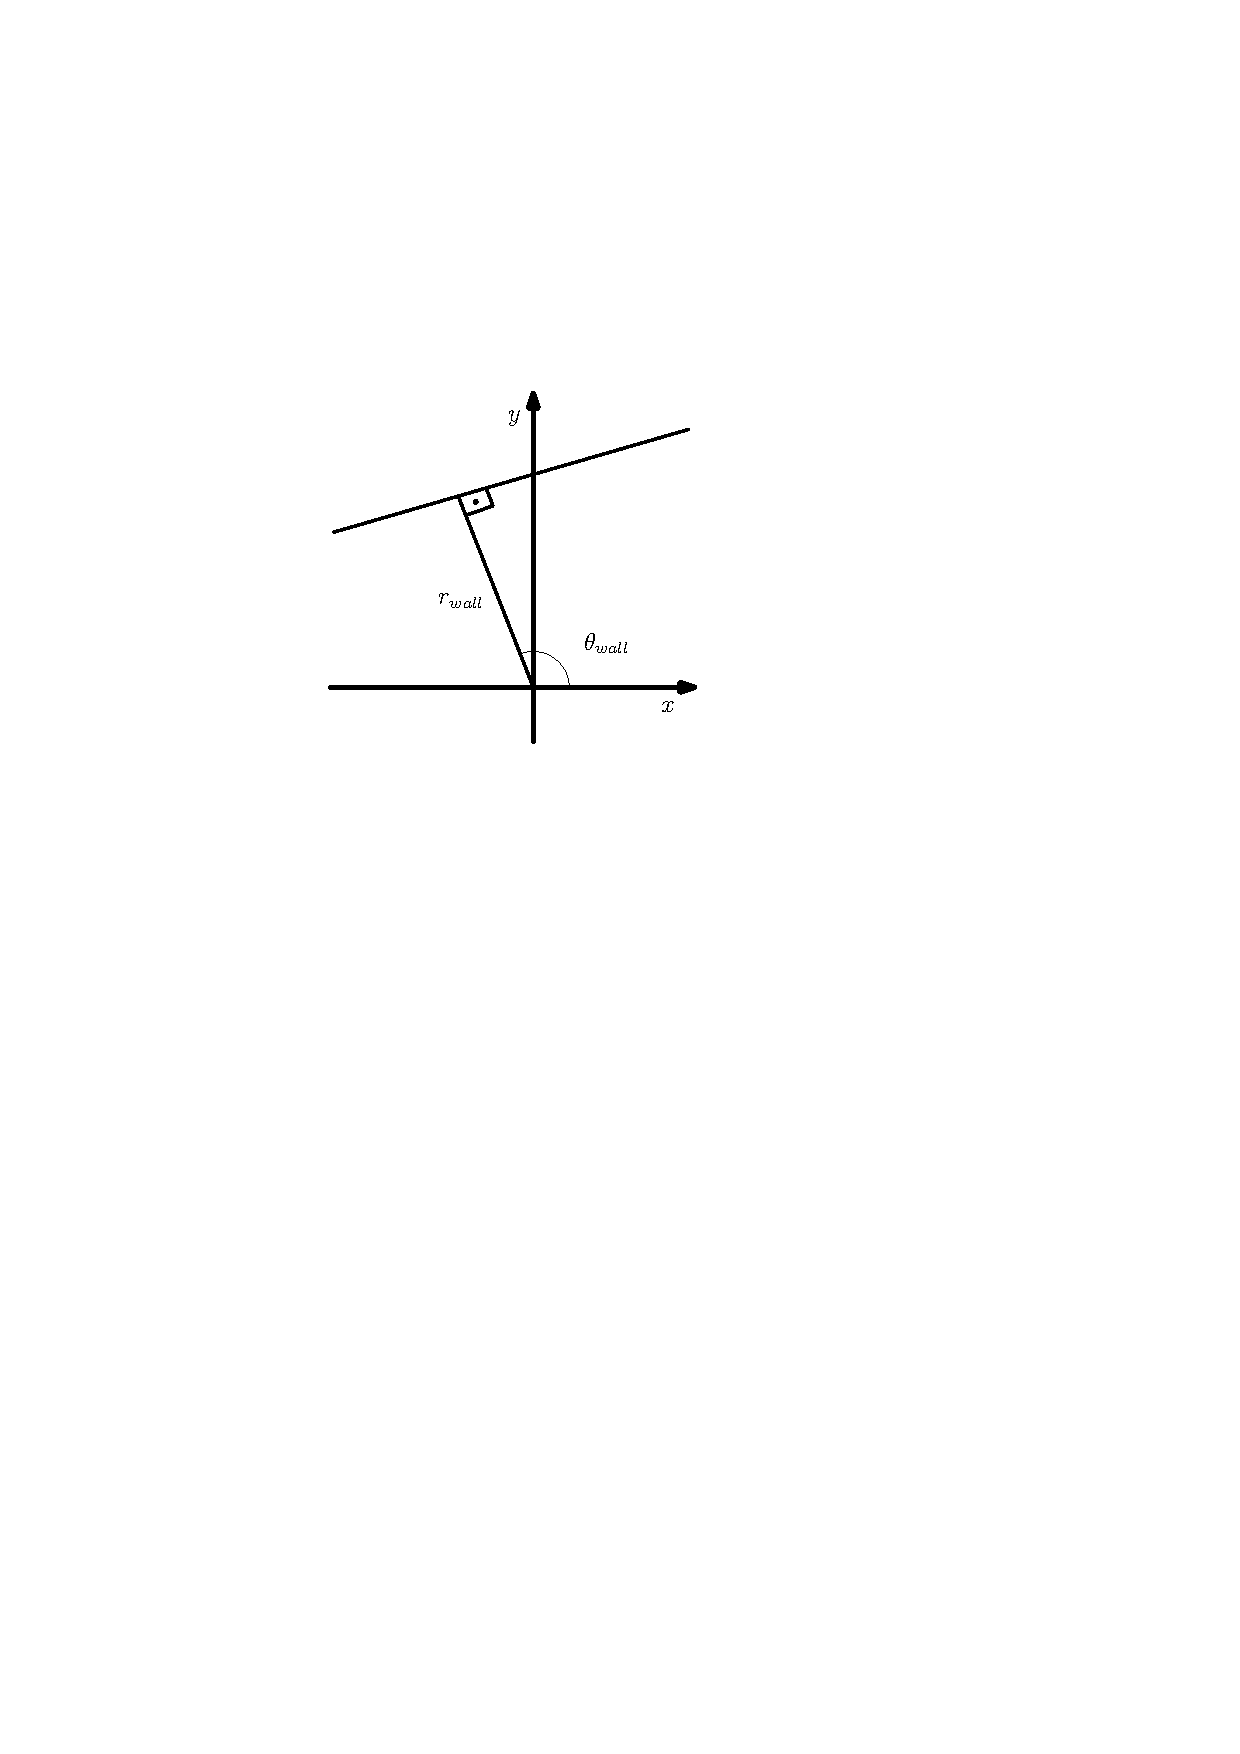
\includegraphics[width=.3\columnwidth]{imagens/retas.pdf}
	\caption{Ilustra��o do modelo adotado para paredes do mapa.}
	\label{fig:retas}
\end{figure}

Note que a divis�o por $\sin\beta$ n�o � problem�tica, pois $\beta$ nunca � m�ltiplo de $\pi$.

Como os tri�ngulos formados entre a posi��o do rob�, o ponto de incid�ncia do feixe do sonar na parede e a intersec��o da traget�ria do rob� com a parede possuem sempre os mesmos �ngulos, independentemente do tempo, podemos usar semelhan�a de tri�ngulos para obter a seguinte equa��o:
\begin{equation}
	\frac{y_{2}-y_{1}}{d_{2,1}}=\frac{y_{3}-y_{2}}{d_{3,2}}=\frac{y_{k}-y_{k-1}}{d_{k,k-1}}
\end{equation}
E considerando que:
\begin{equation}
	\frac{y_{j,j-1}}{d_{j,j-1}}=\gamma_{j,j-1}
\end{equation}
formamos um conjunto com todos os elementos $\gamma_{j,j-1}$ com $j>1$ e $j \leq k$.

Assumindo-se que um �nico segmento de reta est� sendo observado por todas as observa��es, e que a diferen�a entre duas dist�ncias distintas sejam aproximadamente iguais, podemos considerar que todos os elementos do conjunto formado por $\gamma$ s�o elementos de uma mesma distribui��o.

Assim, para verificar se podemos validar a distribui��o, � usado o seguinte teste de hip�tese:
\begin{equation}
		H_{0}:\gamma ~ N(A, \sigma^{2}_{obsmedia})
\end{equation}
\begin{equation}
		H_{1}:\gamma ~ N(A, \sigma^{2}_{alternativo}), \sigma^{2}_{obsmedia} < \sigma^{2}_{alternativo}
\end{equation}
sendo que o teste � realizado sobre a estat�stica $\chi^{2}$.
Para aceitar $H_{0}$, � verificado se $\chi^{2}$ � menor que um dado limite:
\begin{equation}
	\chi^{2}_{k-2} < \chi^{2}_{k-2,\alpha}
\end{equation}
onde o segundo termo � tabelado e $\alpha$ indica a confian�a no teste e o primeiro termo � obtido da seguinte equa��o:
\begin{equation}
	\chi^{2}_{k-2} = \frac{(k-2)s^{2}_{\gamma}}{\sigma^{2}_{obsmedia}}
\end{equation}
onde $s^{2}_{\gamma}$ � a vari�ncia do conjunto formado por $\gamma$.

As observa��es s�o validadas se o teste acima descrito resulte em sucesso.

Oi, eu estou citando o Barra\cite{barra}.

\addcontentsline{toc}{section}{Refer�ncias} 
\bibliographystyle{plain}
\bibliography{referencias}
\end{document}
